\documentclass[tikz,border=8pt]{standalone}
\usepackage[T1]{fontenc}
\usepackage{tikz}
\usetikzlibrary{calc}

\definecolor{edgecolor}{HTML}{475569}
\definecolor{nodefill}{HTML}{FFFEF5}
\definecolor{nodeedge}{HTML}{0F172A}
\definecolor{subtle}{HTML}{475569}

\tikzset{
  qnode/.style={circle, draw=nodeedge, fill=nodefill, line width=0.8pt, minimum size=6.5mm, inner sep=0pt, font=\sffamily\bfseries\small},
  qedge/.style={draw=edgecolor, line width=1.0pt},
  qtitle/.style={font=\sffamily\bfseries\Large},
  qsubtitle/.style={font=\sffamily\small, text=subtle},
  pagetitle/.style={font=\sffamily\bfseries\fontsize{20}{22}\selectfont},
  footnote/.style={font=\sffamily\small, text=subtle}
}

\newcommand{\drawQOne}{%
  \node[qnode] (a0) at (-1.3,0.9) {0};
  \node[qnode] (a1) at (1.3,0.9) {1};
  \node[qnode] (a2) at (1.3,-1.4) {2};
  \node[qnode] (a3) at (-1.3,-1.4) {3};
  \draw[qedge] (a0) -- (a1);
  \draw[qedge] (a1) -- (a2);
  \draw[qedge] (a2) -- (a3);
  \draw[qedge] (a3) -- (a0);
  \draw[qedge] (a0) -- (a2);
}

\newcommand{\drawQTwo}{%
  \node[qnode] (b0) at (0.0,1.25) {0};
  \node[qnode] (b1) at (-1.25,-0.1) {1};
  \node[qnode] (b2) at (1.25,-0.1) {2};
  \node[qnode] (b3) at (-0.45,-1.8) {3};
  \node[qnode] (b4) at (0.95,-1.8) {4};
  \draw[qedge] (b0) -- (b1) -- (b2);
  \draw[qedge] (b0) -- (b2);
  \draw[qedge] (b0) -- (b3);
  \draw[qedge] (b0) -- (b4);
  \draw[qedge] (b1) -- (b3);
  \draw[qedge] (b2) -- (b3);
  \draw[qedge] (b3) -- (b4);
}

\newcommand{\drawQThree}{%
  \node[qnode] (c0) at (-0.8,1.15) {0};
  \node[qnode] (c1) at (0.8,1.15) {1};
  \node[qnode] (c2) at (-0.55,-0.15) {2};
  \node[qnode] (c3) at (0.55,-0.15) {3};
  \node[qnode] (c4) at (0.0,-1.85) {4};
  \draw[qedge] (c0) -- (c1);
  \draw[qedge] (c0) -- (c2);
  \draw[qedge] (c0) -- (c3);
  \draw[qedge] (c1) -- (c2);
  \draw[qedge] (c1) -- (c3);
  \draw[qedge] (c2) -- (c4);
  \draw[qedge] (c3) -- (c4);
}

\newcommand{\drawQFour}{%
  \node[qnode] (d1) at (-1.5,1.0) {1};
  \node[qnode] (d3) at (1.5,1.0) {3};
  \node[qnode] (d0) at (0.0,-0.25) {0};
  \node[qnode] (d2) at (-1.5,-1.55) {2};
  \node[qnode] (d4) at (1.5,-1.55) {4};
  \draw[qedge] (d1) -- (d3);
  \draw[qedge] (d1) -- (d2);
  \draw[qedge] (d2) -- (d4);
  \draw[qedge] (d1) -- (d0);
  \draw[qedge] (d2) -- (d0);
  \draw[qedge] (d3) -- (d0);
  \draw[qedge] (d4) -- (d0);
}

\newcommand{\drawQFive}{%
  \node[qnode] (e1) at (-1.2,1.2) {1};
  \node[qnode] (e2) at (1.2,1.2) {2};
  \node[qnode] (e0) at (0.0,-0.1) {0};
  \node[qnode] (e4) at (-1.2,-1.7) {4};
  \node[qnode] (e3) at (1.2,-1.7) {3};
  \draw[qedge] (e1) -- (e2) -- (e3) -- (e4) -- cycle;
  \draw[qedge] (e0) -- (e1);
  \draw[qedge] (e0) -- (e2);
  \draw[qedge] (e0) -- (e3);
  \draw[qedge] (e0) -- (e4);
}

\newcommand{\drawQSix}{%
  \node[qnode] (f0) at (-1.0,1.1) {0};
  \node[qnode] (f1) at (1.0,1.1) {1};
  \node[qnode] (f2) at (-1.0,-0.35) {2};
  \node[qnode] (f3) at (1.0,-0.35) {3};
  \node[qnode] (f4) at (0.0,-1.95) {4};
  \draw[qedge] (f0) -- (f1);
  \draw[qedge] (f0) -- (f2);
  \draw[qedge] (f0) -- (f3);
  \draw[qedge] (f0) -- (f4);
  \draw[qedge] (f1) -- (f2);
  \draw[qedge] (f1) -- (f3);
  \draw[qedge] (f1) -- (f4);
  \draw[qedge] (f2) -- (f3);
  \draw[qedge] (f3) -- (f4);
}

\begin{document}
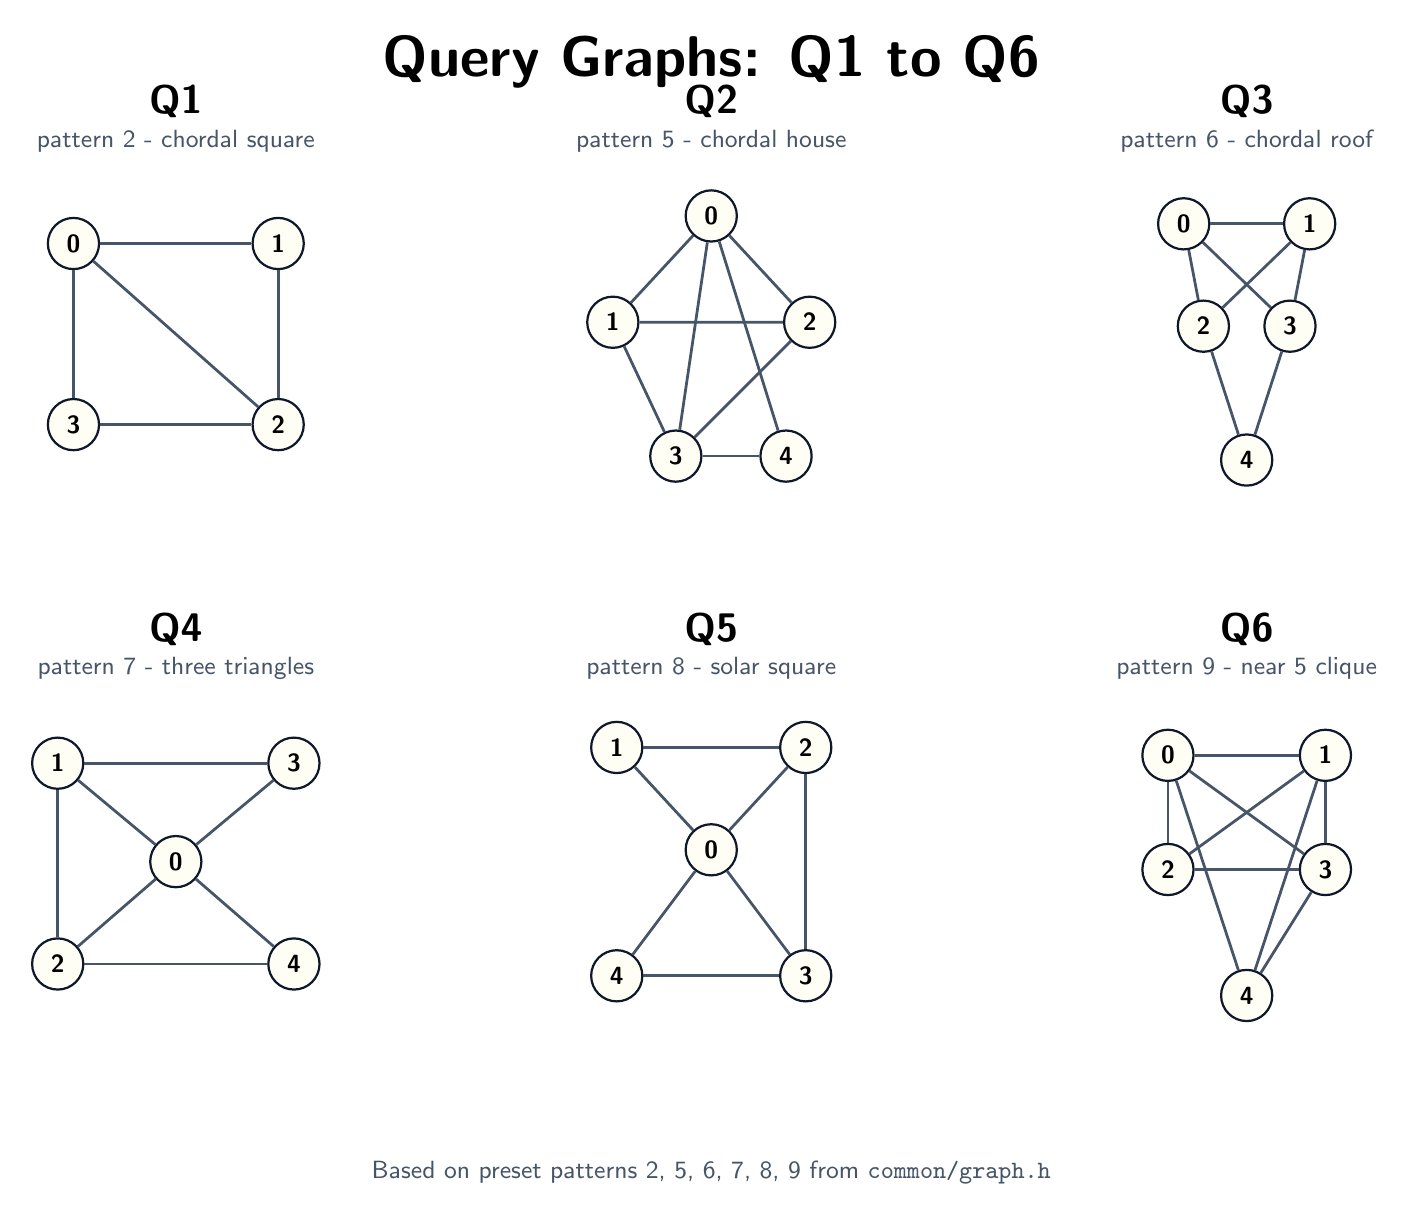
\begin{tikzpicture}[x=1cm,y=1cm]
  \node[pagetitle] at (0,4.9) {Query Graphs: Q1 to Q6};

  \begin{scope}[shift={(-6.8,1.7)}]
    \node[qtitle] at (0,2.7) {Q1};
    \node[qsubtitle] at (0,2.2) {pattern 2 - chordal square};
    \drawQOne
  \end{scope}

  \begin{scope}[shift={(0,1.7)}]
    \node[qtitle] at (0,2.7) {Q2};
    \node[qsubtitle] at (0,2.2) {pattern 5 - chordal house};
    \drawQTwo
  \end{scope}

  \begin{scope}[shift={(6.8,1.7)}]
    \node[qtitle] at (0,2.7) {Q3};
    \node[qsubtitle] at (0,2.2) {pattern 6 - chordal roof};
    \drawQThree
  \end{scope}

  \begin{scope}[shift={(-6.8,-5.0)}]
    \node[qtitle] at (0,2.7) {Q4};
    \node[qsubtitle] at (0,2.2) {pattern 7 - three triangles};
    \drawQFour
  \end{scope}

  \begin{scope}[shift={(0,-5.0)}]
    \node[qtitle] at (0,2.7) {Q5};
    \node[qsubtitle] at (0,2.2) {pattern 8 - solar square};
    \drawQFive
  \end{scope}

  \begin{scope}[shift={(6.8,-5.0)}]
    \node[qtitle] at (0,2.7) {Q6};
    \node[qsubtitle] at (0,2.2) {pattern 9 - near 5 clique};
    \drawQSix
  \end{scope}

  \node[footnote] at (0,-9.2) {Based on preset patterns 2, 5, 6, 7, 8, 9 from \texttt{common/graph.h}};
\end{tikzpicture}
\end{document}
